% ---
% Capitulo de revisão de literatura
% ---



\chapter{Revisão Bibliométrica sobre Filtragem de dados de sensores}\label{referencial_teorico}

Nesta seção são consideradas as informações referentes à produção acadêmica mundial, que abordam os termos em inglês Noise reduction, noise abatement, Filtering algorithm e Sensor, significando em sequência redução de ruído, algoritmos de filtragem e sensores.

Ambos os tópicos foram pesquisados na base IEEE Xplore, com a busca limitada aos termos noise reduction e noise abatement no título do documento e filtering algorithm, sensor e noise reduction apenas no texto completo, delimitando exclusivamente aos artigos de 2018 a 2022. Resultando em 675 resultados sendo eles 450 conferências, 215 artigos, 8 artigos com acesso  antecipado e 2 revistas, foi realizado uma revisão bibliométrica sobre estes 215 artigos resultantes.

Dados oriundos de sensores são constantemente bombardeados com interferências aleatórias do ambiente onde se encontram, também devido a baixa qualidade provenientes dos sensores de baixo custo disponíveis, inserindo valores incorretos que são caracterizados como ruídos nas amostras. Esse problema desperta um grande interesse de pesquisadores, que buscam lidar com o tratamento e a filtragem de dados ruidosos provindos de sensores diversos, o artigo \cite{chiang_noise_reduction_in_ECG} se destaca por ser o trabalho mais citado nessa pesquisa bibliométrica, o mesmo aborda o problema da interferência de ruídos nos sinais provindos dos sensores de eletrocardiograma, esses dados podem ser contaminados por fatores como a estática da pele ou mesmo pela respiração do paciente, para isso técnicas como wavelet são muito populares, utilizadas para filtrar dados cancelando o ruído analisando mudanças bruscas ou picos na frequência do sinal, o método de decomposição do modo empírico também é bastante utilizado, definindo fronteiras entre o local máximo e mínimo de uma subtração de sequência que consequentemente ajudam na triagem do tratamento do sinal.

\begin{figure}[H]
	\centering
	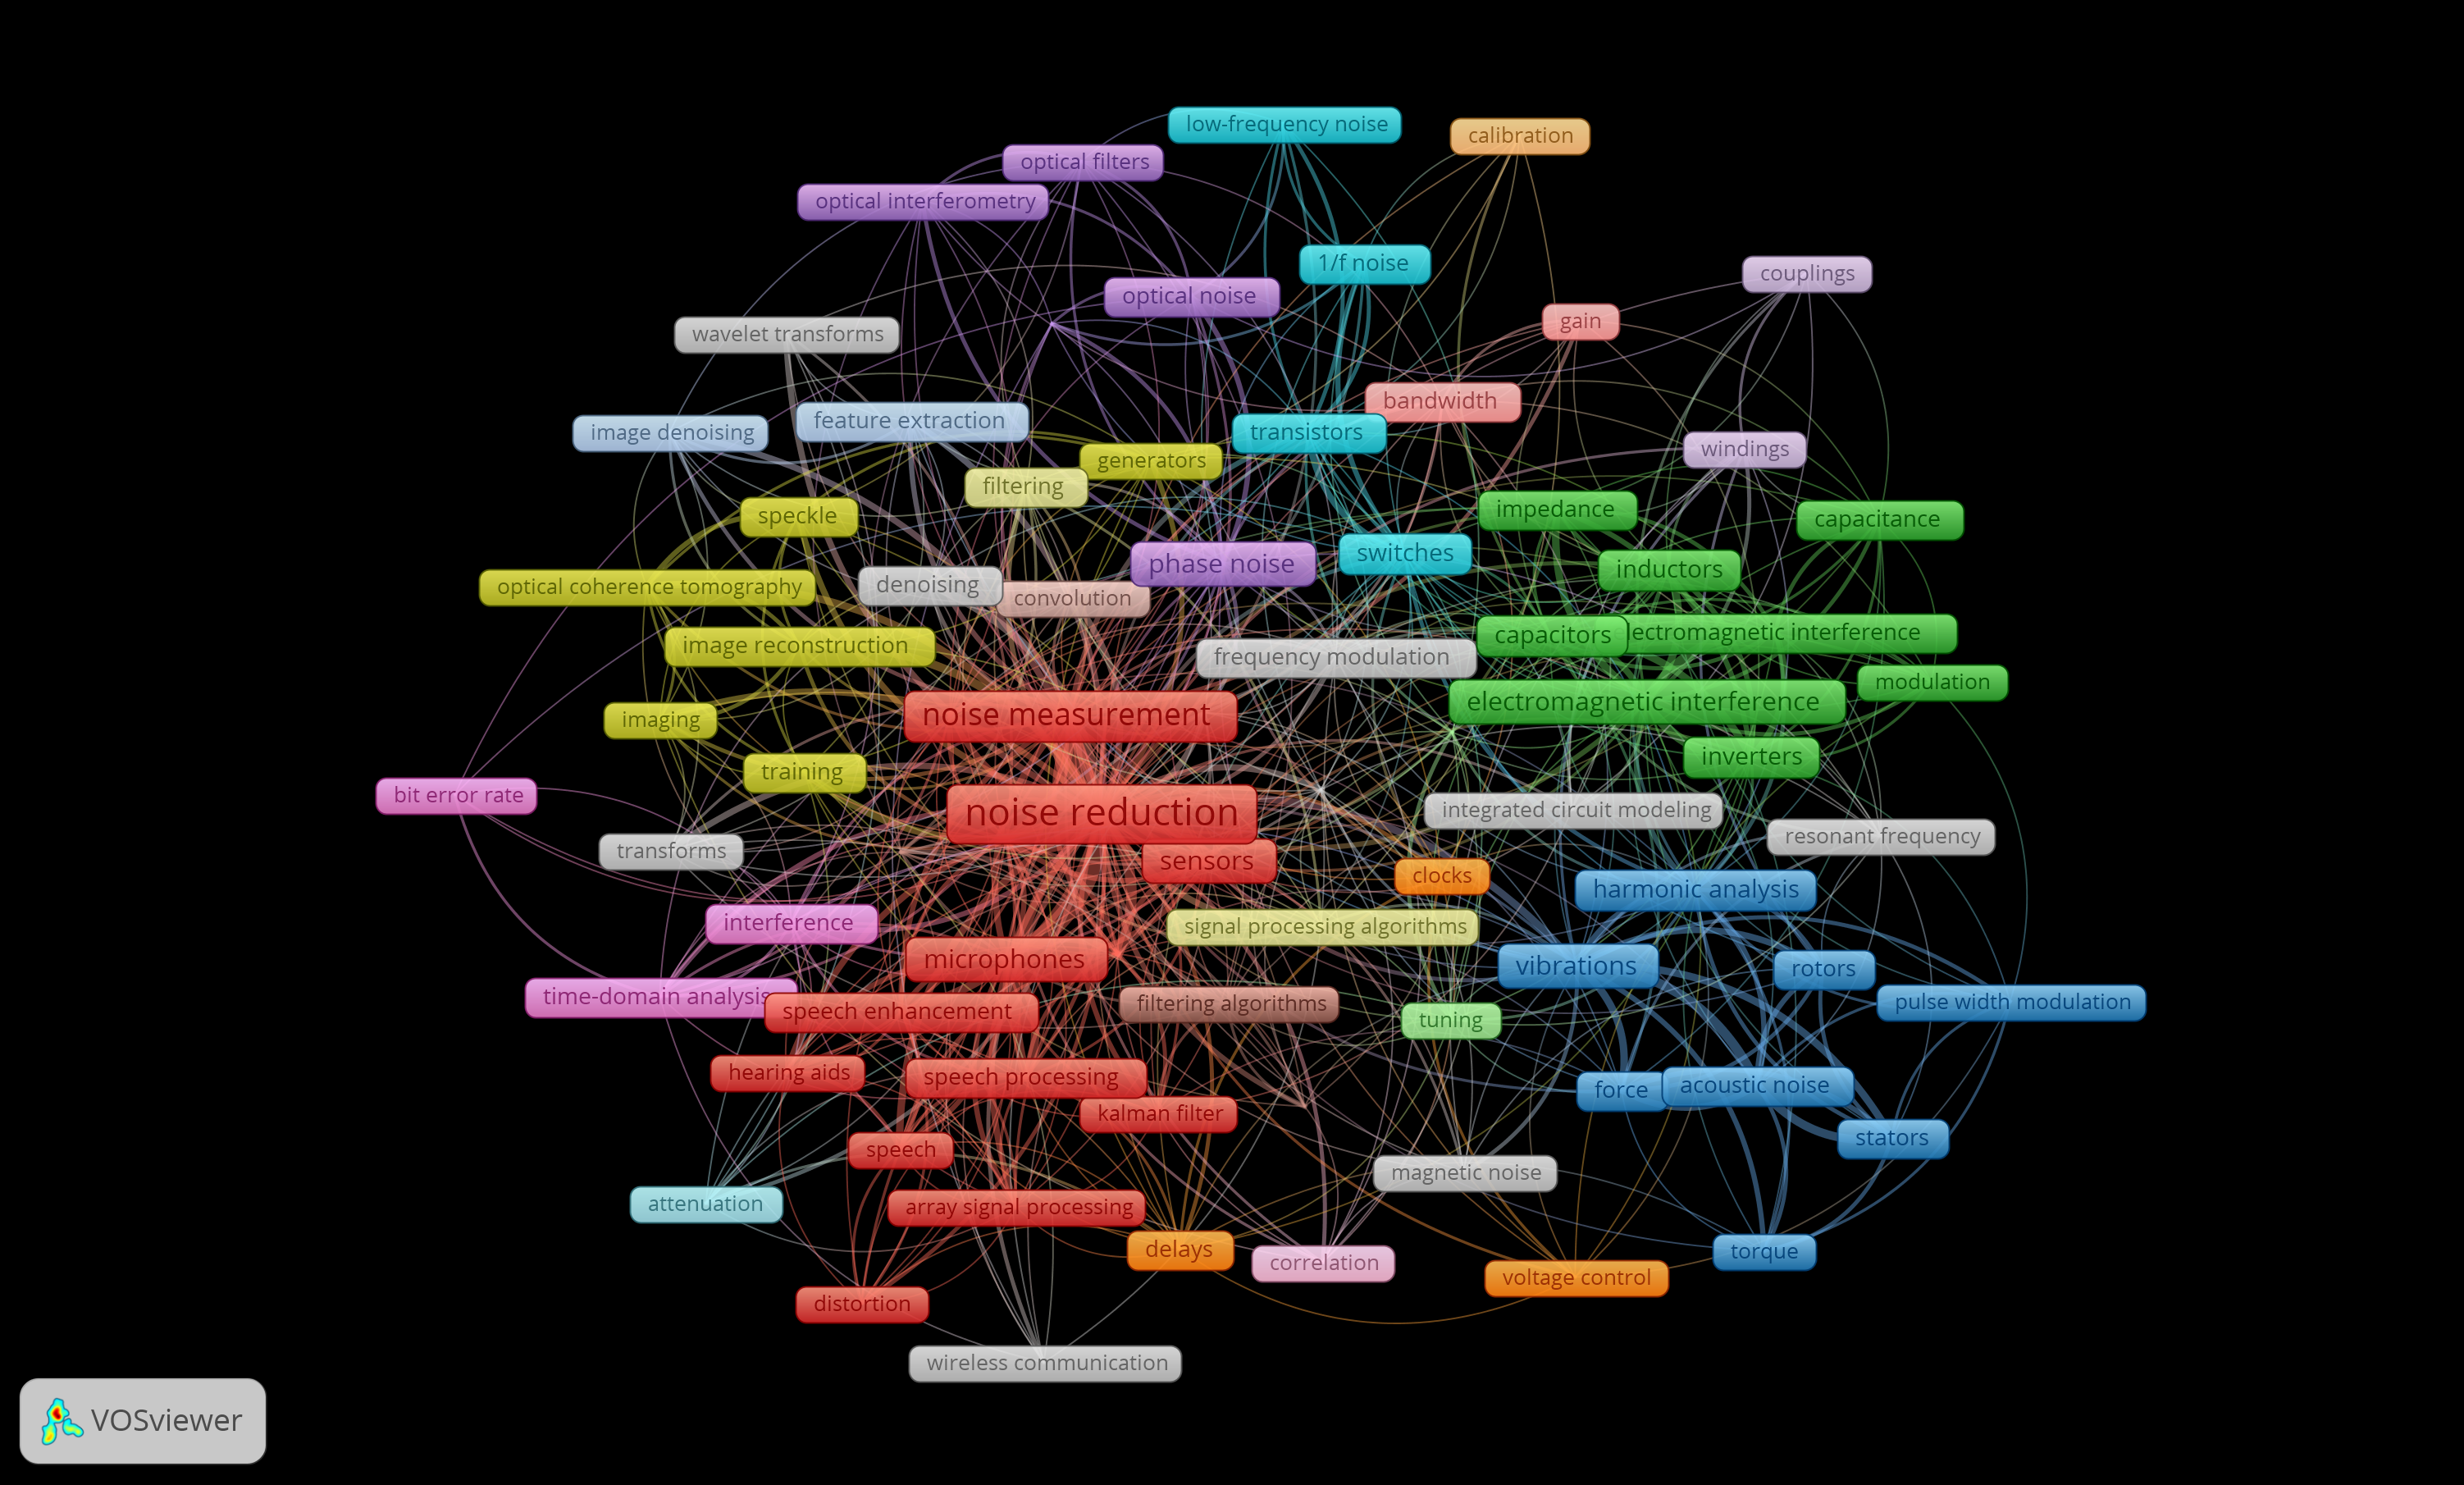
\includegraphics[width=\textwidth,height=\textwidth]{anexos/ris/IEEE/Noise_reduction_and_noise_abatement_andsensor_filtering_algorithm/network_visualization_with_lines.png}
	\caption{Mapa de visualização de rede}
	Fonte: Autor com base no Software VOSViwer.
	\label{fig: network_visualization_with_lines}
\end{figure}

A Figura~\ref{fig: network_visualization_with_lines} representa um mapa de visualização de rede, onde pode-se visualizar os termos mais predominantes. Aqui são percebidos o termos que se repetiram mais de 5 vezes nos textos e resumos, nota-se a formação de grupos de acordo com suas áreas de atuação, alguns termos em destaque são em azul relacionados a motores, vibrações e forças mecânicas, os em verdes referentes a componentes eletrônicos, roxo a sensores ópticos, amarelo o tratamento de imagem e em vermelho sensores embarcados e processamento de sinais. 


Todas essas expressões aprofundam a problemática no qual tratamento de ruídos, algoritmos de filtragem e sensores estão correlacionados, indo de problemas em programas de computador a desenvolvimento de circuitos eletrônicos e peças mecânicas. O erro na fabricação de sensores ópticos pode levar a fenômenos de interferência nos resultados \cite{liu_interference_stripe}, essas anomalias prejudicam sistemas de medição holográfica digital, a fim de melhorar a captação de imagens sem ruído o autor propõem um novo método de processamento de imagem utilizando pirâmide laplaciana para destacar o ruído de faixa de interferência.

\begin{figure}[H]
	\centering
	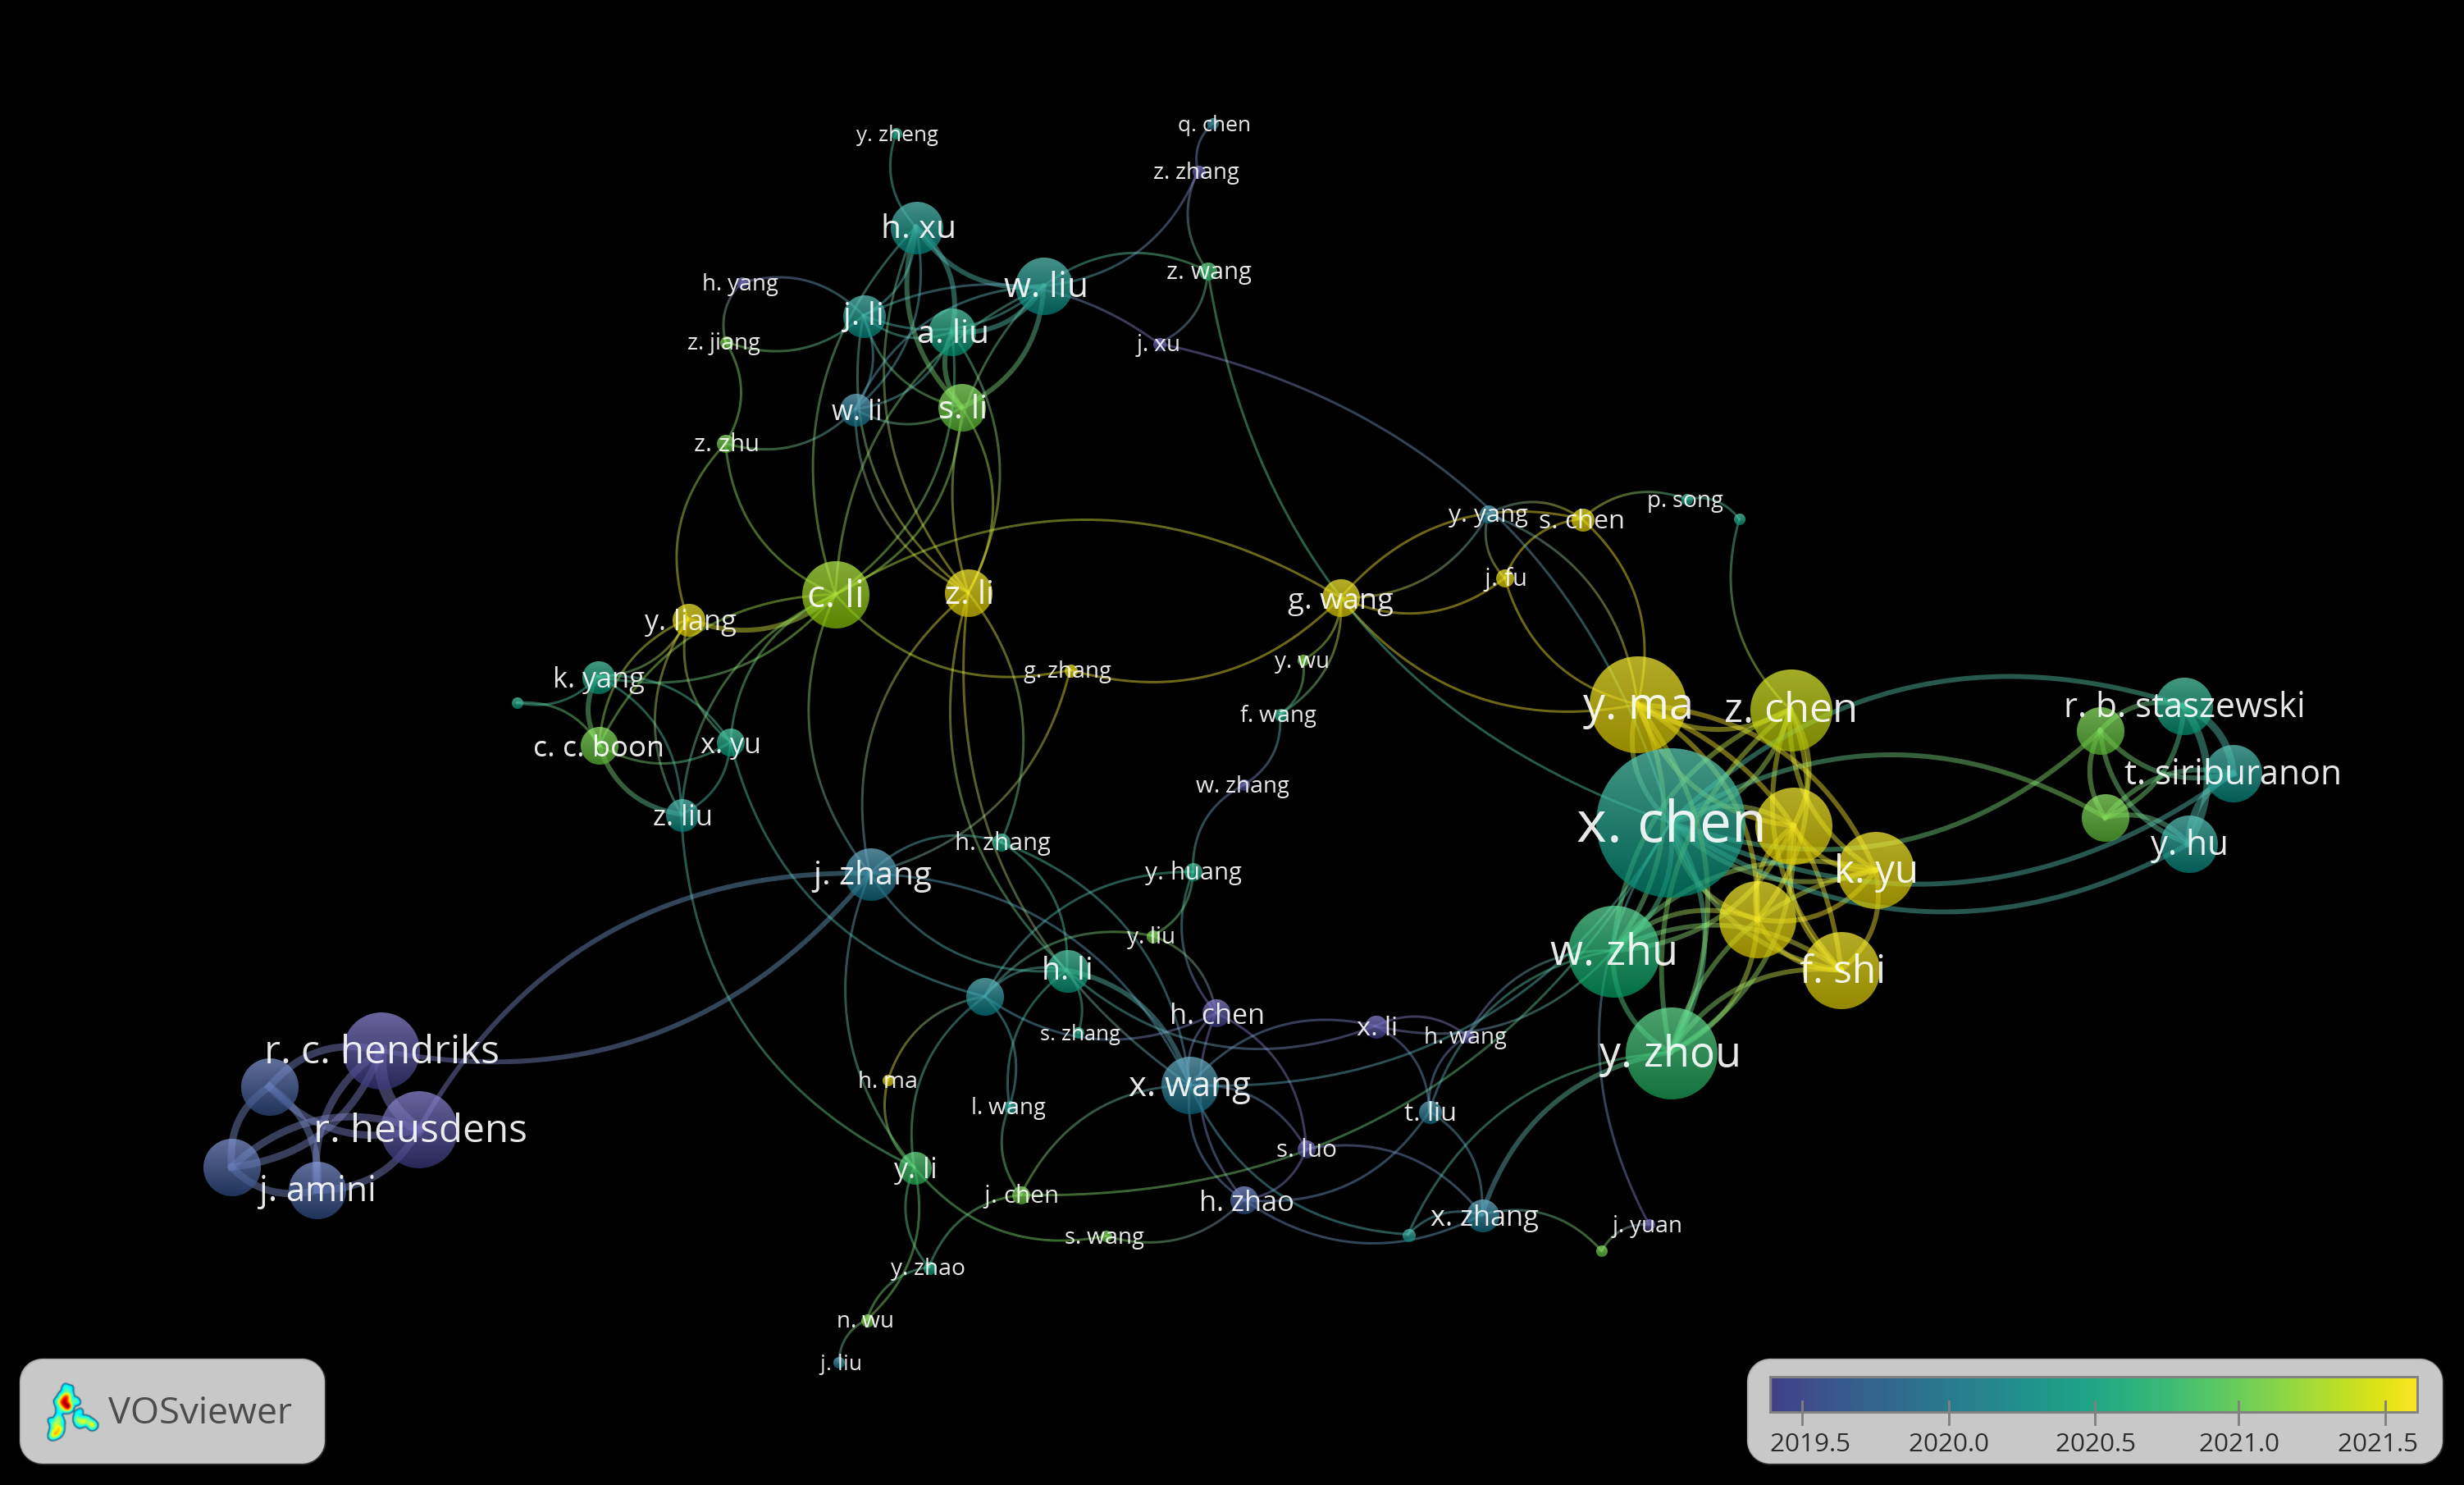
\includegraphics[width=\textwidth,height=\textwidth]{anexos/ris/IEEE/Noise_reduction_and_noise_abatement_andsensor_filtering_algorithm/overlay_visualization_cites.png}
	\caption{Mapa de visualização autores}
	Fonte: Autor com base no Software VOSViwer.
	\label{fig: overlay_visualization_cites}
\end{figure}

A Figura~\ref{fig: overlay_visualization_cites} apresenta um mapa semelhante a figura anterior, a imagem destaca os autores mais citados em média, destacando-os pelo tamanho do círculo atrás de seu nome, e pela sua presença em artigos mais recentes de acordo com a cor mais amarelada.
Em \cite{duarte_speckle_noise} afim de melhorar aplicações biomédicas em imagens de ultrassom, o trabalho descreveu 27 técnicas para tratamento eliminação de ruído para ultrassom, essas imagens são de verdadeira importância para o diagnóstico clínico e procedimentos terapêuticos não invasivos, fundamentais em diversas áreas da saúde.

Na Figura~\ref{fig: overlay_visualization} abaixo visualiza-se um mapa de sobreposição, onde os vocabulários mais amarelos representam os que se encontram em publicações em média mais recentes, também podemos notar a relação entre as palavras encontradas em todos os títulos e resumos.

\begin{figure}[H]
	\centering
	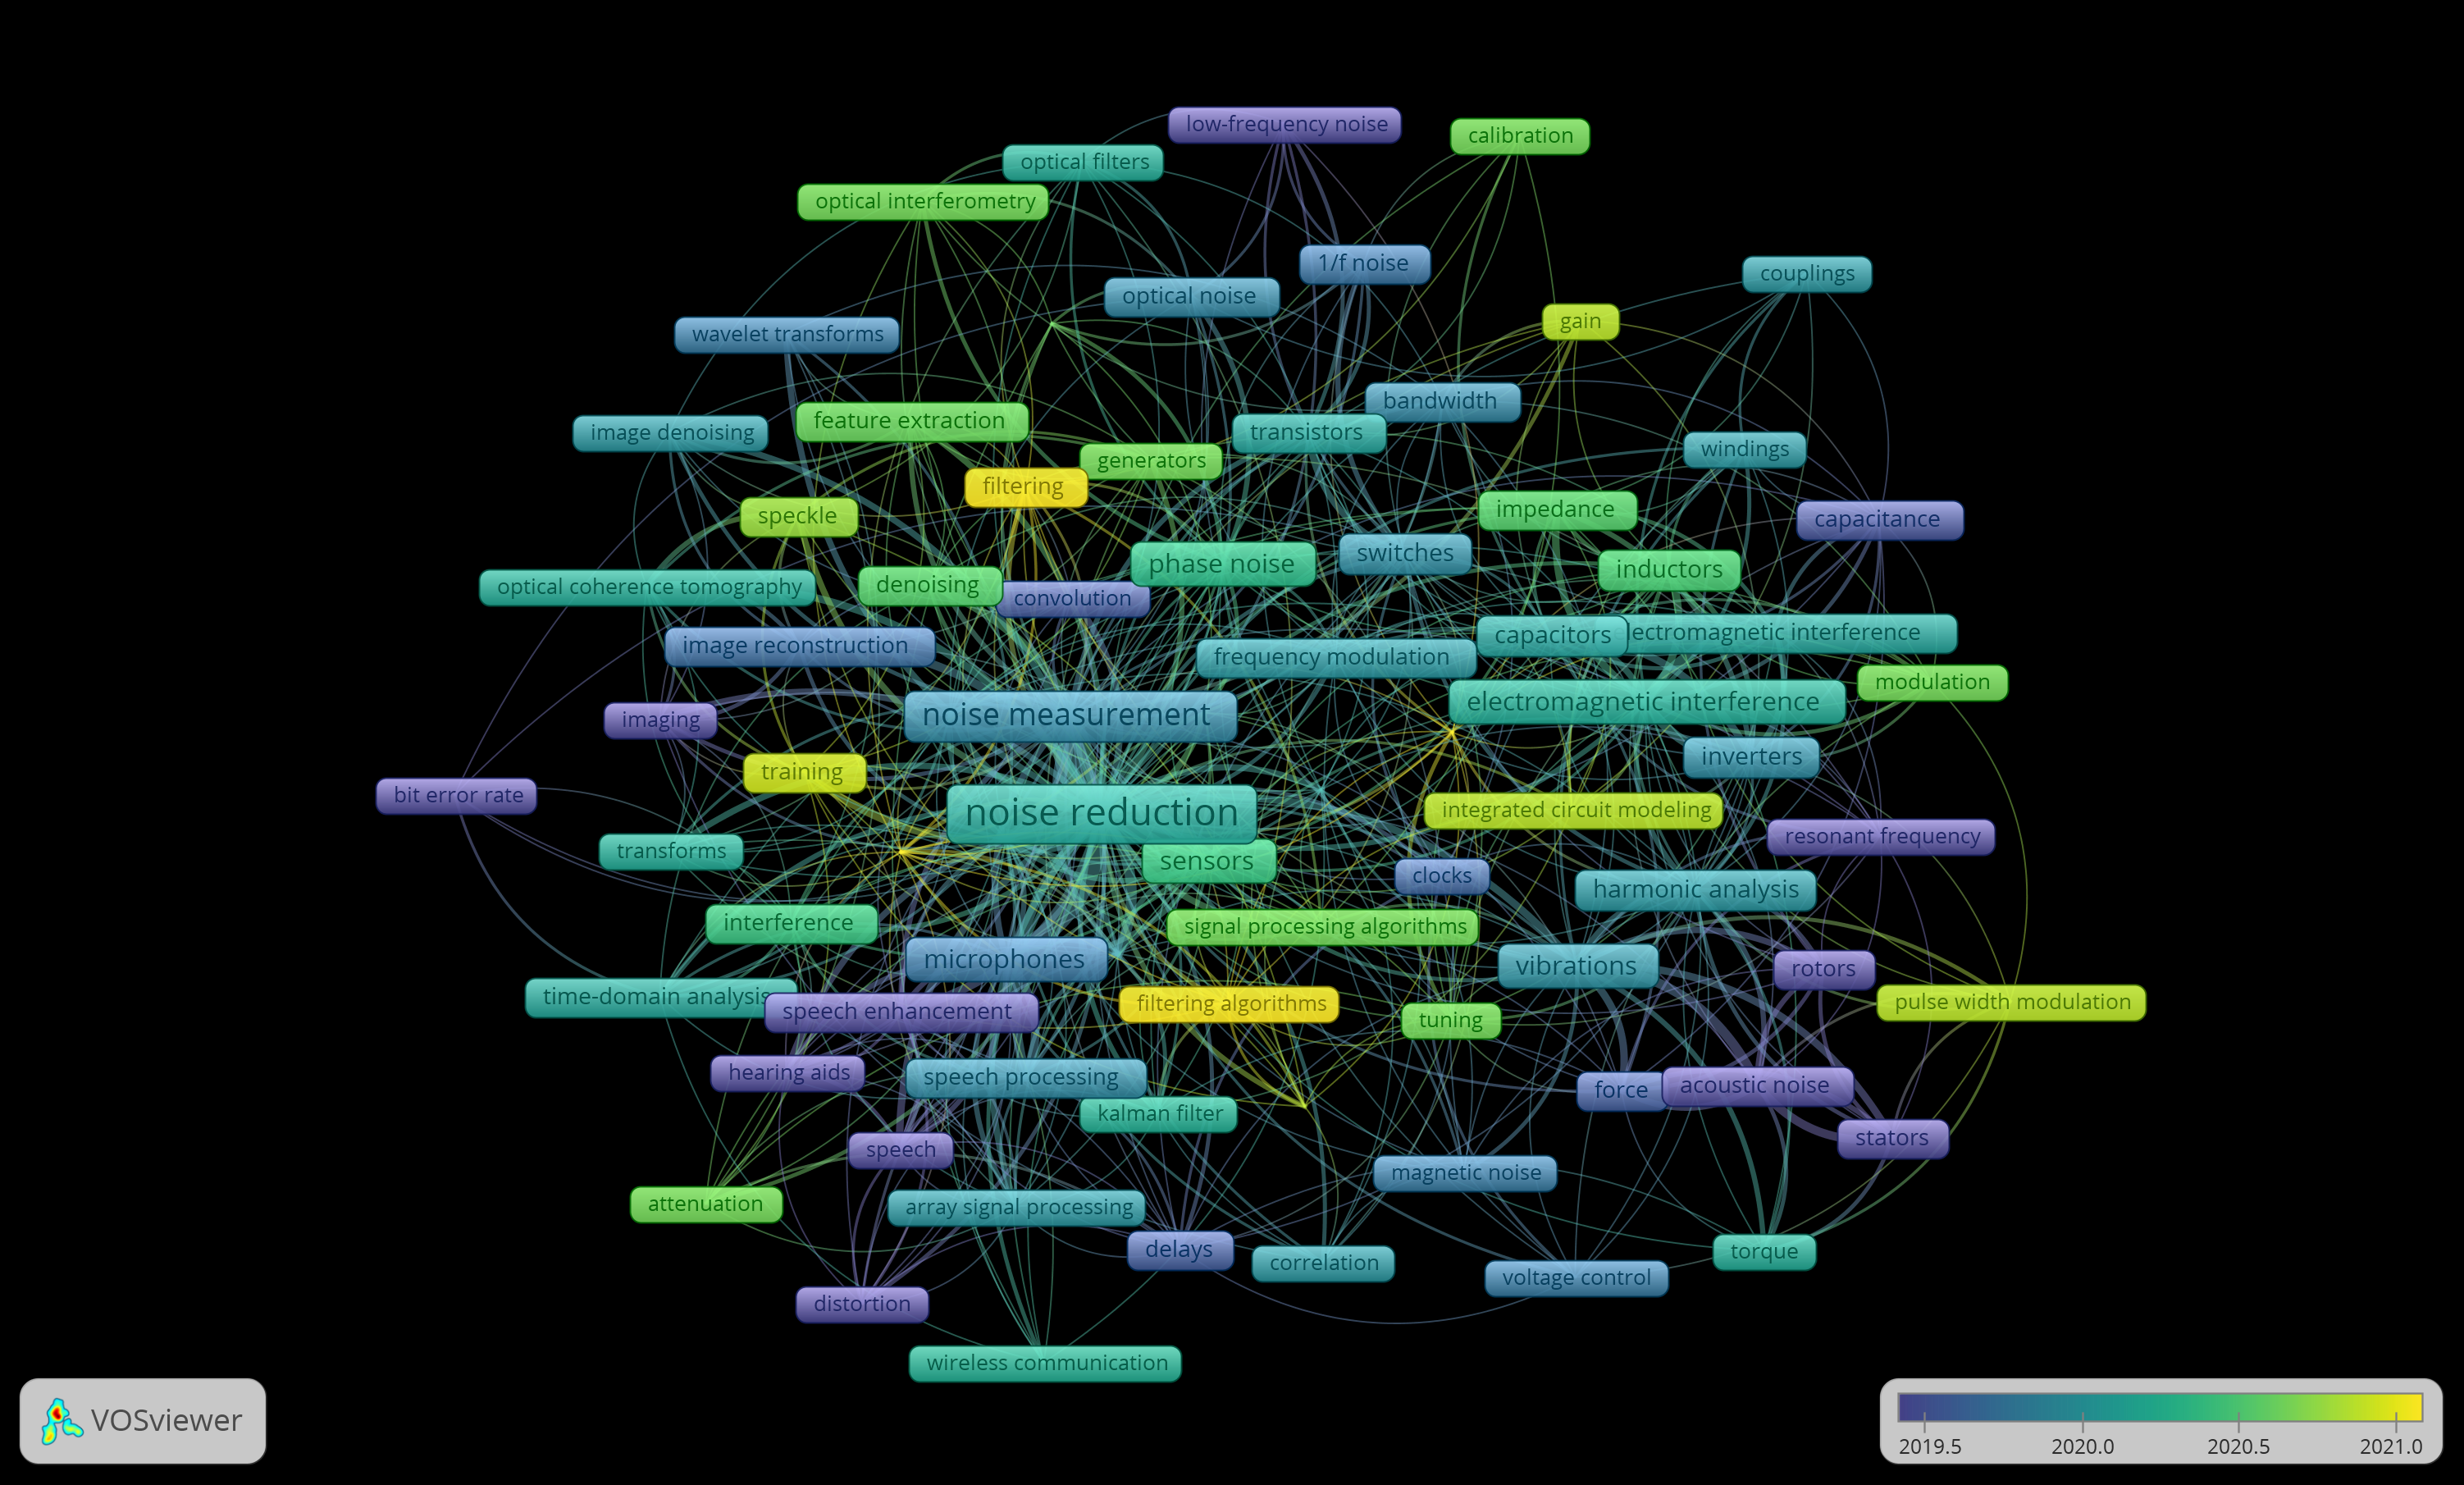
\includegraphics[width=\textwidth,height=\textwidth]{anexos/ris/IEEE/Noise_reduction_and_noise_abatement_andsensor_filtering_algorithm/overlay_visualization.png}
	\caption{Mapa de sobreposição}
	Fonte: Autor com base no Software VOSViwer.
	\label{fig: overlay_visualization}
\end{figure}

Há de se notar que os termos filtragem e algoritmos de filtragem se destacam pela sua quantidade acima da média de trabalhos mais recentes, não se distanciando das definições de redução de ruído, sensores e algoritmos de processamento de sinais próximos do centro do mapa.
 


\subsection{Conclusões sobre a Revisão Bibliométrica realizada}
Percebe-se que o estudo na área de tratamento de dados de sensores concentra em média uma grande quantidade de trabalhos recentes, com diferentes abordagens de como remover ou reduzir dados ruidosos, apresentando a ideia de que o tema é de interesse atual da comunidade acadêmica mundial. A diversos ramos nos quais tratamento e eliminação de ruídos de sensores podem peregrinar, podendo verificar a ocorrência dos termos em problemas que não necessariamente estão interessados na obtenção do sinal limpo, mas sim na caracterização e coleta dos ruídos na amostra ou que fogem do escopo deste trabalho com a eliminação de ruído, sendo feita através de equipamento físico.



\section{Trabalhos Relacionados}%\label{referencial_teorico}
% Aqui será dedicado a descrever os trabalhos relacionados ao tema desta pesquisa.

O trabalho \cite{kalambet2011noise} descreve um método de filtragem de ruído baseado em intervalo de confiança, com uma abordagem que utiliza matrizes para evitar dados discrepantes deixando-os como estão, o estudo enfatiza alguns dos problemas encontrados nos filtros mais utilizados, como a falta de critério claro da filtragem e interferência no resultado final. 

A pesquisa \cite{madhale2020adaptive} apresenta uma técnica de remoção de ruído adaptável baseada em intervalo de confiança adaptável e orientado a dados, para limpeza de valores do monitoramento através de eletroencefalograma que analisa a atividade elétrica cerebral espontânea, o trabalho obteve sucesso reduzindo significamente as taxas de ruído tornando a dinâmica do cérebro mais analisável no exame e com menos interferência.
\pagebreak
\subsection{Tabela de referencias}
Aqui serão apresentados os 5 artigos recentes relacionados a esse trabalho, tendo suas vantagens e desvantagens levantadas com relação aos seus métodos propostos e uma breve descrição do trabalho.

\begin{longtable}{|p{2cm}|p{4cm}|p{3.5cm}|p{3.5cm}|}
    \hiderowcolors
    \caption{Referências bibliográficas}
    \label{tab:makespan}\\
    \showrowcolors
    \hline
    \rowcolor[HTML]{C0C0C0} 
    \multicolumn{1}{c|}{\cellcolor[HTML]{C0C0C0}\textbf{Trabalhos analisados}} & \multicolumn{1}{c|}{\cellcolor[HTML]{C0C0C0}\textbf{Objetivo}} & \multicolumn{1}{c|}{\cellcolor[HTML]{C0C0C0}\textbf{Vantagens}} & \multicolumn{1}{c|}{\cellcolor[HTML]{C0C0C0}\textbf{Desvantagens}} \\ \hline

    \endfirsthead
    \rowcolor[HTML]{C0C0C0} 
    \multicolumn{1}{c|}{\cellcolor[HTML]{C0C0C0}\textbf{Trabalhos analisados}} & \multicolumn{1}{c|}{\cellcolor[HTML]{C0C0C0}\textbf{Objetivo}} & \multicolumn{1}{c|}{\cellcolor[HTML]{C0C0C0}\textbf{Vantagens}} & \multicolumn{1}{c|}{\cellcolor[HTML]{C0C0C0}\textbf{Desvantagens}} \\ \hline

    \endhead
    \hline
    \cite{Arab_LSTM_ResNet} &   O trabalho propõe utilizar uma técnica de aprendizado profundo para classificar e eliminar ruídos de sistemas de comunicação via micro-ondas, aproveitando-se da aptidão do algoritmo em se adestrar se com os dados coletados em tempo real.	& Algoritmo pode ser treinado em tempo real e acompanhar diferentes tipos de ruídos. & Necessita de uma grande quantidade de dados já coletados para treinamento, exigência de grande capacidade de recurso de computação. \\ \hline
   
    \cite{Kamata_mems} &   O seguinte estudo propõe uma filtragem para processamento de sinal de um componente eletrônico giroscópio embarcado e avaliando seu desempenho. &   A técnica pode ser utilizada também para acelerômetros, e viabiliza o uso de componentes de custo baixo e alta precisão. & Limitasse a um ambiente de sensores específicos. \\ \hline
    
    \cite{Ning_magnetometer} &   Aqui os autores implementam uma combinação de filtros para eliminar dados ruidosos em tempo real e compensar a interferência dos erros de um sensor magnético, utilizando de diversos métodos como Auto-Regressão e Média móvel, para modelar a medição de ruído, a fim de excluir dados errados do resultado final. &   O método utilizado é adaptativo e abrangente, podendo resolver ruídos dinamicamente. & Os testes não foram realizados durante o processo de coleta de dados. \\ \hline
    
    \cite{Kaan_emg} &   Aqui é proposto um novo método de processamento de dados de sensores de eletromiografia sensível, utilizando um algoritmo adaptativo em tempo real para eliminar os ruídos provindos de fontes elétricas de corrente alternada, sem perturbar os dados reais do sensor, ao qual conseguiu superar cinco alternativas existentes de última geração para tratamento de sinal de eletromiografia, mantendo a qualidade do sinal.  &  Seu comportamento adaptativo exibe uma vantagem em manter os dados coletados o mais próximo possível dos dados reais, sem diminuir a potência do sinal. & Por estar no estado da arte, ainda não apresenta outros estudos comprovando sua utilização em tempo real. \\ \hline
    
    \cite{Zhou_ambient} &   Os autores apresentam um método que combina processamento de sinal e cancelamento de ruído adaptativo para filtrar e eliminar interferências do ambiente. Duplicando o sinal recebido em dois canais diferentes, sobrepondo um sobre o outro e eliminando as interferências em ambos de forma a evitar perdas dos espectros. &   Identifica sinais de interferência utilizando uma quantidade inferior de dados. & Quanto maior a sobreposição, maior a carga computacional necessária para processar os canais diferentes. \\ \hline
    
\end{longtable}
 

% Ademais, 
% o levantamento bibliométrico passa a ideia que utilizar Zephyr em um projeto de Cubesat não 
% e uma ideia muito distante, abrindo uma janela de possíveis trabalhos na área que possam 
% trazer grandes contribuições, possibilitando o surgimento deste trabalho.

% Conclusão


% \subsection{Problema da interferência em sensores}

\section{Intervalo de confiança}
Segundo \cite{patino2015intervalos} um IC é a metade da divisão do tamanho do real efeito na população de interesse, essa imprecisão ou diferença entre duas médias é sempre a melhor estimativa dado o tamanho da população atingida. De acordo com \cite{henriques2011dificuldades} o intervalo de confiança é um dos procedimentos gerais de inferência estatística que pode aplicar-se a diversos campos de problemas. Os mais utilizados são estimação de parâmetros desconhecidos de uma população, comparação de distribuições, teste de hipóteses sobre parâmetros populacionais, determinar o tamanho de amostra adequado para realizar uma inferência, e determinar limites de tolerância. Cada um destes campos é muito alargado e variado e incluem a estimação de média, proporção, variâncias, parâmetros de regressão e correlação.  


\section{ Filtro de Kalman}

O filtro é baseado em probabilidade estatística sendo capaz de suavizar ruídos de sensores eletrônicos visando seu posterior processamento \cite{International_Conference__Zhuang}.


\cite{tan2005sensoclean} diz que através de uma sequência de dados observados o filtro de Kalman pode estimar o estado verdadeiro de um sistema dinâmico, o mesmo é utilizado por uma grande parte das aplicações de engenharia que visam sistemas complexos como visão computacional ou radares. 
 

\section{Média Móvel}
De acordo com \cite{santos2021educaccao}, a média móvel é uma técnica que consiste em calcular a média aritmética das observações mais recentes de uma série de dados temporais. Portanto, temos uma estimativa que não leva em consideração a observação mais antiga. Os autores também esclareceram que o nome média móvel foi usado porque a cada período as observações mais antigas são substituídas pelas mais recentes, então uma nova média é calculada.


\section{Média Móvel Ponderada}
Segundo \cite{ribeiro2020analise}, a média móvel ponderada é superior à média móvel simples porque realiza uma mudança de impacto entre os dados de demanda mais antigos e os mais recentes, o que pode revelar algumas tendências. Eles também afirmam que a média móvel simples atribui o mesmo peso a cada componente da série de dados, enquanto a média móvel ponderada permite atribuir um fator de ponderação a cada elemento onde a soma de todos os pesos é igual a um.



% \section{Filtro FIR}

% \section{Filtro IIR}
